\subsubsection{\large{Cервис запуска расчётных задач}}
\addcontentsline{toc}{subsubsection}

Детальная архитектура сервиса запуска расчётных задач представлена на диаграмме компонент
(см. рис\ \ref{pic:architecture__orchestrator-component}).

\begin{figure}[H]
	\hspace*{-2.5 cm}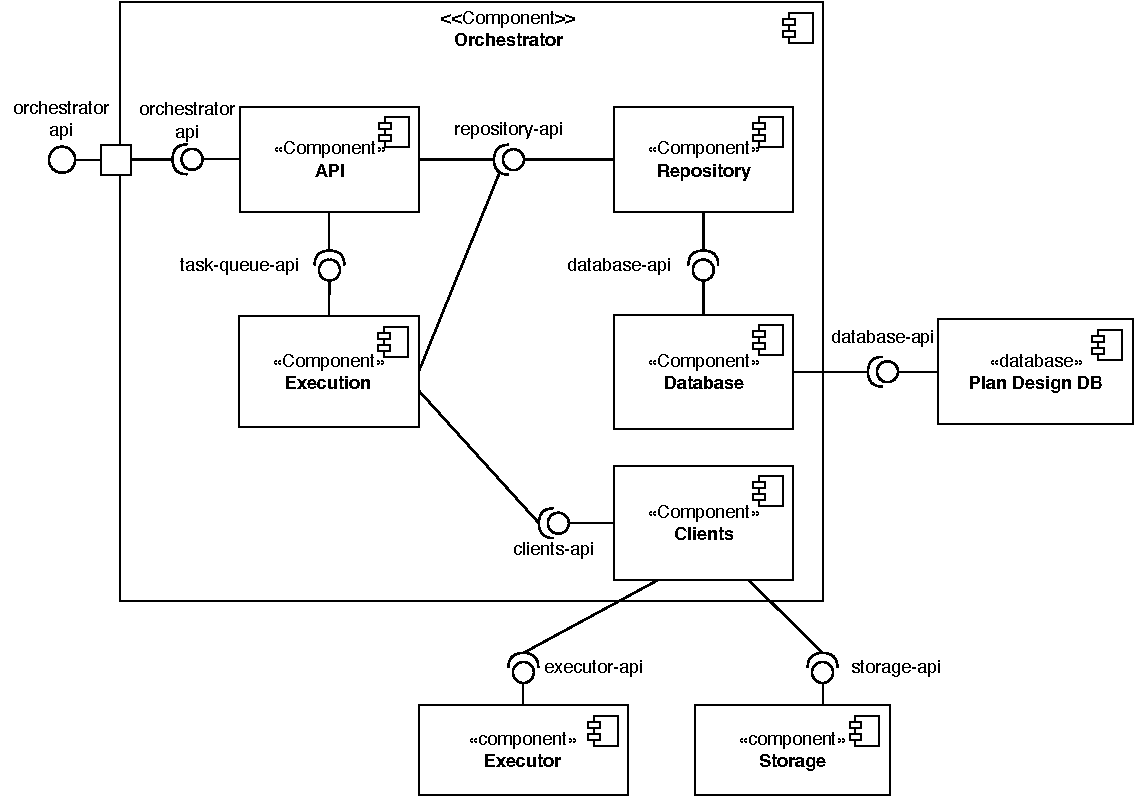
\includegraphics[width=\textwidth]{architecture/pictures/orchestrator/component_common}
	\caption{Диаграмма компонент сервиса запуска расчётных задач}
	\label{pic:architecture__orchestrator-component}
\end{figure}
\vskip 5 mm

Сервис представлен следующими компонентами:
\begin{enumerate}
	\item {
		\textit{API} -- отвечает за предоставление REST API и отправки задачи в очередь.
	}
	\item {
		\textit{Repository} -- отвечает за получение и сохранение данных и логику их преобразований.
	}
	\item {
		\textit{Execution} -- компонент, отвечающий за выполнение расчётных задач.
	}
	\item {
		\textit{Clients} -- клиенты для взаимодействия с хранилищем расчётных данных
		и сервисом запуска математических методов.
	}
	\item {
		\textit{Database} -- чтение/сохранение сущностей базы данных.
	}
\end{enumerate}

Для расчёта генерального плана площадного объекта в автоматическом режиме используются четыре типа сущностей,
представленные на диаграмме ниже(см. рис.\ref{pic:architecture__orchestrator-classes})
\begin{figure}[H]
	\hspace*{-2.5 cm}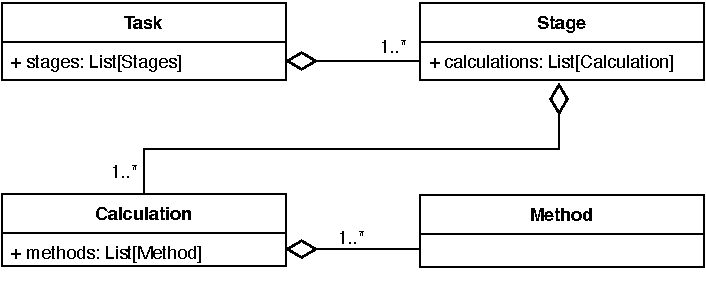
\includegraphics[width=\textwidth]{architecture/pictures/orchestrator/classes}
	\caption{Диаграмма классов}
	\label{pic:architecture__orchestrator-classes}
\end{figure}
\vskip 5 mm

\begin{itemize}
	\item {
		\textit{Task} -- расчётная задача. Задача состоит из набора этапов, которые выполняются последовательно.
	}
	\item {
		\textit{Stage} -- этап расчётной задачи. Для каждого этапа определена хотя бы одна последовательность
		математических методик.
	}
	\item {
		\textit{Calculation} -- последовательность математических методик.
	}
	\item {
		\textit{Method} -- запуск математической методики, представленной в математической библиотеке.
	}
\end{itemize}



Самой технически сложной частью сервиса является компонент, отвечающий за запуск расчётных задач.
Детальное изображение его компонентов представлено
на диаграмме ниже (см. рис\ \ref{pic:architecture__orchestrator-detailed-component}).

\begin{figure}[H]
	\hspace*{-2.5 cm}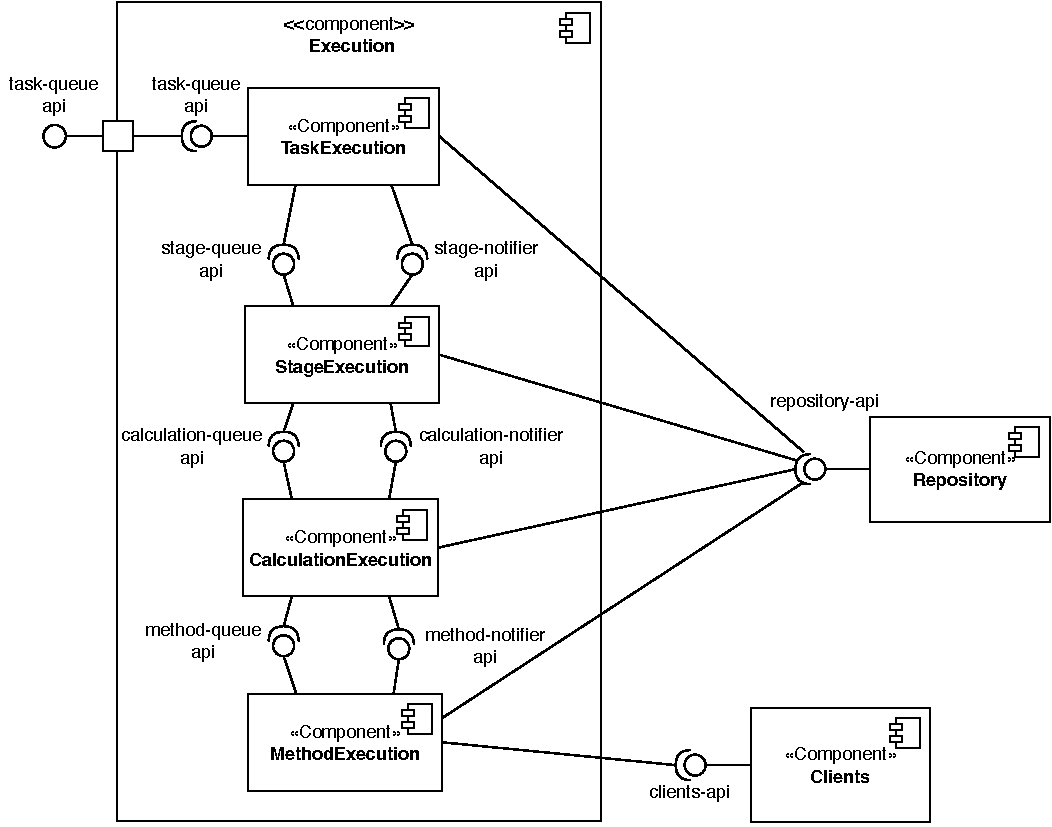
\includegraphics[width=\textwidth]{architecture/pictures/orchestrator/component_detailed}
	\caption{Диаграмма компонент сервиса запуска расчётных задач}
	\label{pic:architecture__orchestrator-detailed-component}
\end{figure}
\vskip 5 mm


Сервис представлен следующими компонентами:
\begin{enumerate}
	\item {
		\textit{Task Execution}
	}
	\item {
		\textit{Stage Execution}
	}
	\item {
		\textit{Calculation Execution}
	}
	\item {
		\textit{Method Execution}
	}
\end{enumerate}
